\documentclass[12pt,MSc,wordcount,anon]{muthesis}
\usepackage{verbatim}
\usepackage{graphicx}
\usepackage{hyperref}
\usepackage{listings}
\usepackage{pslatex}
\usepackage{rotating}
\begin{document}

\title{A Consistency Analysis of Pathogenicity Prediction Methods for \textit{In Silico} Generated Nonsynonymous Single Nucleotide Polymorphisms}
\author{Samuel Acosta-Melgarejo}
\stuid{10232284}
\principaladviser{Michael Cornell}
\faculty{Faculty of Biology, Medicine and Health}
\department{}

\begin{flushleft}
\urlstyle{sf}

\beforeabstract
\prefacesection{Abstract}
\input{abstract}
\afterabstract

\prefacesection{Acknowledgements}
This work was done at the Division of Evolution and Genomic Sciences of the School of Biological Sciences of the University of Manchester, under the supervision of Dr Michael Cornell, for whose guidance and support I am immensely grateful. The project was part of the Bioinformatics and Systems Biology master's programme, for which I was sponsored by Chevening Scholarships, the UK government's global scholarship programme, funded by the Foreign and Commonwealth Office (FCO) and partner organisations.
\afterpreface

\clearpage
\begin{flushright}
    \thispagestyle{empty}
    \vspace*{\fill}
    A mis padres.
    \vspace*{\fill}
\end{flushright}
\clearpage

\chapter{Introduction}
\label{cha:intro}

Recent developments in molecular genetics, along with the extended use of Next Generation Sequencing technology and the increasing availability of molecular data as a result of scientific efforts in diverse fields and with different interests, have had a profound impact in medicine and biology. They have transformed the fields of clinical diagnosis and population genetics, and led to the development of fields such as personalised medicine and biomedical engineering. Improvements in quality and volume of biological data have required the widespread use of computational techniques to support research and model complex biological interactions in almost every step of the research process.

A particularly important and practical type of computational tools used in bioinformatics is prediction methods. They are increasingly used in the biosciences to forecast diverse features and characteristics (Vihinen, 2012). In genetic testing and similar sequencing projects, genes with mutated sequences are frequently detected, and a challenging task consists in predicting the level of pathogenicity that these sequences have for the organism.

There are several possible types of mutations, as a result of the different possible changes in the nucleotides that form the DNA sequence. A \textit{missense} mutation occurs when a single amino acid of a translated protein is replaced for a different one. These mutations are mostly the result of \textit{single nucleotide polymorphisms} (SNPs), which are the most common form of genetic variation in humans (Thusberg et al., 2011). They are nonsynonymous nucleotide substitutions occurring within a protein-coding region of a genome for a fraction of a particular population. They are referred to as \textit{single nucleotide variants} (SNVs) when they are considered independently of the rest of a population.

The different types of mutations differ in terms of their potential harmfulness for the organisms. A \textit{nonsense} mutation, for example, is likely to be pathogenic, because it could cause the premature termination of translation and protein synthesis. Some of the mutations caused by SNPs are responsible for Mendelian diseases and some are not, so their pathogenicity is difficult to predict (Pshennikova et al., 2019). An important and challenging task is to find prediction methods to distinguish variants that have a negative effect on protein functions from those that do not in the most accurate way possible.

Computational methods are used in diagnostic laboratories together with other lines of evidence like allele frequency in a population and family history. However, current guidelines establish that the classification of variants as disease-causing of benign cannot be based on computational methods alone, and that they could only be taken as supporting evidence (Richards et al., 2015). For this reason, many variants are classified as variants of uncertain significance (VUS).

Computational tools are widely used to perform this task (Niroula and Vihinen, 2019). There are several different approaches to the design of these tools, and they are frequently tested and compared to assess which ones are more precise and useful. Survey and benchmarking efforts about the existing methods can be found in Dong et al. (2015), Peterson et al. (2013), Pshennikova et al. (2019), Suybeng et al. (2020), Tang and Thomas (2016), Thusberg et al., (2011) and Walters-Sen et al. (2015). Most studies emphasise the correct identification of deleterious variants. A work focused on benign variants detection is performed in Niroula and Vihinen (2019).

With new methods and approaches emerging constantly, there have been efforts to provide advice on how to critically select the appropriate methods for particular needs in Vihinen (2012) and Niroula and Vihinen (2016). There are also tools that incorporate several methods and produce and ensemble-like score to try to take advantage of each method's capabilities, like the ones presented in Kircher et al. (2014) and Dong et al. (2015). Lastly, in the set of practice guidelines for the evaluation of pathogenicity published by the Association for Clinical Genetic Science, a section is dedicated to \textit{in silico} pathogenicity predictors, where it is stated, among other things, that: 1) the tool generating the optimal predictive score will depend upon the gene under investigation and parameters used; 2) the analysis of a particular variant should be performed using at least three different programmes, and users should ideally use tools based on different algorithms; and 3) the classification generated from the prediction tools must not be considered definitive and must form one aspect of a wider investigation (Wallis et al., 2013).

The pathogenicity prediction methods can be classified following different criteria. One possible way of grouping them is taking into account the type of information that is given more importance when building the predictions. Following this criteria, a distinction could be done between methods that emphasise the importance of the evolutionary information and those that incorporate other types of biological information. In the first case, the predictions are primarily based on the principle that mutations that result in diseases or have a negative impact on the organisms would have most likely reduced the organisms' fitness in the evolutionary process, and consequently would not be retained. The opposite would have happened with mutations that were benign, which would have been more likely to pass to subsequent generations. Because of this, high frequencies of variants indicate benignness, and the opposite, harmfulness (Niroula and Vihinen, 2019). Most of these methods use multiple sequence alignments from orthologous sequences to detect conserved amino acids. The conservation of an amino acid that is over a wide range of species is used to indicate that changes at that position have been selected against. In the second case, the tools try to incorporate several other types of biological information to build prediction scores, for example, functional annotations, the GC content of the molecules, and all kinds of other biological features. A separate group of predictions methods could be composed of ensemble-like tools. These methods try to act as meta-predictors joining as many methods as possible and weighing each one according to certain criteria, incorporating methods mostly based on evolutionary data and others using all types of biological data.

Despite all the guidelines and benchmarking work among all the different approaches, a particular problem that emerges in the assessment of these methods is that they often provide contradictory pathogenicity information for the same variants. This is mostly due to the use of curated datasets of known pathogenicity in the development and testing of the tools. These datasets have the disadvantage of being very disproportionate in the distribution of observations among different sets of genes. For example, genes as BRCA1 and BRCA2 have much richer datasets that other less-studied genes, with many more confirmed disease-causing variants. This causes biases in the assessment of the methods that tend to overestimate their performance. A detailed work concerning the measurement of these biases and the challenges concerning them can be found in Grimm et al. (2015).

The present work had the aim of exploring, contrasting and analysing pathogenicity prediction patterns and trends provided by different approaches and methods, for a computationally generated dataset, composed of all the possible missense variants caused by SNPs, for a sample set of genes. Particularly, the project aims to examine these patterns and trends in the light of other measures and biological features (external to the pathogenicity predictors) like sequence position, empirical values of missense changes tolerance observed in the genes, and amino acid replacement measures. In addition, the project aimed to provide a computational tool to support this research, that could serve as a standalone, user-oriented application, with the capability to reproduce and extend the results of this project in an easy and automated way.

The project used a different approach from that of most of the cited literature. As described above, rather than using a curated dataset as a reference for a pathogenicity prediction assessment of the methods, an artificial dataset composed of the complete set of possible SNP-caused mutations for a set of genes was computationally created. Then, an exploratory approach was taken to identify patterns and trends existing among the results of a representative set of methods, comparing their partial and global predicted deleteriousness values with external measurements. This approach was selected for several reasons. First, it allows for a high volume comparison of deleteriousness prediction values that is difficult to obtain using datasets of known pathogenicity, due to the limitations described. Moreover, it avoids the problems of circularity and bias in the predictions that arise from the use of these datasets.

Only nonsynonymous mutations possibly caused by SNPs were considered due to the fact that their frequency is much greater than changes that could only be caused by the substitution of 2 or 3 nucleotides in the DNA sequence.

Lastly, SNiPtool, a web-based software application for the generation and analysis of artificial SNP-caused variants, was developed and made available. It was designed with the reproducibility of the results in mind, and with the potential of generating the complete dataset on demand for an arbitrary set of genes using web-based services.


\chapter{Materials and Methods}
\label{cha:methods}

\section{Genes and Transcripts}

To build the dataset of possible SNP-caused variants, 15 human known disease-causing genes, associated with breast cancer and colon cancers, were selected (ATM, BRCA1, BRCA2, CHEK2, TP53, MLH1, MRE11, MSH2, MSH6, NBN, PALB2, PMS2, RAD50, RAD51 and XRCC2). The genes have a diverse range of sequence lengths (843 to 10257 nucleotides length).

The Matched Annotation from NCBI and EMBL-EBI (MANE) curated transcripts were selected as the transcripts to use for variants generation. As opposed to other similar efforts like RefSeq, GENCODE, Consensus Coding Sequence (CCDS) and Locus Reference Genomic (LRG), using the MANE transcripts had the advantage of providing: 1) always just one transcript for each gene (as opposed to RefSeq/GENCODE); 2) values for a great proportion of genes by combining automatic and manual curation (as opposed to the more restrictive CCDS and LRG); and 3) a relatively easy way to retrieve the updated mappings. Version GRCh38.v0.9 of the MANE repository was used. The corresponding transcripts used are shown in Table 1.

\begin{table}
\begin{center}
\begin{tabular}{|r|r|}\hline\hline
Gene&MANE Transcript\\\hline
ATM&ENST00000675843\\
BRCA1&ENST00000357654\\
BRCA2&ENST00000380152\\
CHEK2&ENST00000404276\\
MLH1&ENST00000231790\\
MRE11&ENST00000323929\\
MSH2&ENST00000233146\\
MSH6&ENST00000234420\\
NBN&ENST00000265433\\
PALB2&ENST00000261584\\
PMS2&ENST00000265849\\
RAD50&ENST00000378823\\
RAD51&ENST00000267868\\
TP53&ENST00000269305\\
XRCC2&ENST00000359321\\\hline\hline
\end{tabular}
\end{center}
\caption{MANE transcripts used for each gene}\label{wombat}
\end{table}

\section{Pathogenicity Prediction Methods}

The pathogenicity prediction methods used in the study were selected based on: 1) their diversity of approaches and design principles; 2) their popularity (at least two of them, SIFT and PolyPhen-2, are frequently used by diagnostic labs); and 3) their availability through web-based services that could be integrated in an automated way. To get access to the tools, the Database for Nonsynonymous SNPs' Functional Predictions (dbNSFP) was used (Liu et al., 2016). The dbNSFP is a database that focuses on SNPs' functional prediction, and provides precomputed values for many prediction methods and other tools in a centralised way. Version 4.0a of the database was used, which has values computed until May, 2019.

\subsection{Methods Based on Evolutionary Information}

To obtain the results based on this type of tool, three prediction methods were selected. Sorting Tolerant From Intolerant (SIFT) is one of the most widely used pathogenicity prediction methods. It presumes that important amino acids will be conserved in the protein family, and so changes at well-conserved positions tend to be predicted as deleterious (Ng and Henikoff, 2003).

The Protein Variation Effect Analyzer (PROVEAN) was developed to refine the predictions of in-frame insertions, deletions and multiple amino acid substitutions, and it is also based on an alignment-based score that measures the change in sequence similarity of a query sequence to a protein sequence homolog (Choi et al., 2012).
LRT uses a likelihood ratio test, which compares the probability of the data under a conserved model, allowing for any level of selective constraint, relative to a neutral model, where there is no difference between the nonsynonymous and synonymous substitution rate (Chun and Fay, 2009).

Prediction values for SIFT were retrieved directly from the VEP, using version 5.2.2 of the tool. Values for PROVEAN and LRT were retrieved from the dbNSFP, using versions 1.1 (Jan 2015) and Nov 2009, respectively.

\subsection{Methods Based on Multiple Features}

For this group, five methods were selected. PolyPhen-2 (PPH2) is another very widely used tool to predict pathogenicity. It uses several sequence-based and structure-based predictive features, most of them involving a comparison of a property of the wild-type (ancestral, normal) allele and the corresponding property of the mutant (derived, disease-causing) allele. It then selects a set of homologous sequences using a clustering algorithm and constructs and refines a multiple alignment (Adzhubei et al., 2010). Version 2.2.2 was used, provided by the Ensembl VEP.

MutationTaster2 (MT2) integrates information from different biomedical databases such as UniProt, ClinVar, phyloP and ExAC, analyses comprise evolutionary conservation, splice-site changes, loss of protein features and changes that might affect the amount of mRNA. Test results are then evaluated by a naive Bayes classifier, which predicts the disease potential (Schwarz et al., 2010). Version 2015 was used, provided by dbNSFP.

Functional Analysis Through Hidden Markov Models (FatHMM) does an initial multiple sequence analysis which is used to build a Hidden Markov Model, and then introduces "pathogenicity weights" derived from the relative frequencies of disease‐associated and functionally neutral amino acid substitutions mapping onto conserved protein domains (Shihab et al., 2013). Version v2.3 was used, provided by dbNSFP.
MutPred uses inter-species pairwise alignments along with neural networks trained on datasets like the Human Gene Mutation Database, SwissVar and dbSNP to calculate the probability of the pathogenicity of the variants (Pejaver et al., 2017). Version 1.2 was used, provided by dbNSFP.

Lastly, the Variant Effect Scoring Tool (VEST) uses a machine learning approach, based on the Random Forest supervised algorithm and trained on a positive class of missense variants from the Human Gene Mutation Database and a negative class of common missense variants detected in the Exome Sequencing Project population (Carter et al., 2013). Version 4.0 was used, provided by dbNSFP.

\subsection{Ensemble Prediction Methods}

Three methods were selected to represent this type of approach. The two last methods, MetaSVM and MetaLR are closely related.

Combined Annotation-Dependent Depletion (CADD) is probably the most complex method of the set. It combines more than 60 genomic features with several pathogenicity and conservation scores, and then uses a machine learning model trained on a binary distinction between simulated de novo variants and variants that have arisen and become fixed in human populations since the split between humans and chimpanzees (Rentzsch et al., 2019). Version 1.4 was used, provided by dbNSFP.

MetaSVM and MetaLR are the two ensemble scoring methods provided by the dbNSFP database. They combine 10 different pathogenicity methods for which whole-exome data are available with the use of machine learning models, and they differ in that the first one uses a using a support vector machine and the second one, logistic regression (Dong et al., 2015).

\section{Harmfulness Index}

Individual values of pathogenicity were gathered from each method and combined in a global value, the Harmfulness Index (HI), an index developed for this project. This value was calculated for each variant and summarised following different criteria to explore both possible correlations existing between the method's predictions and external measurements and to show the variable levels of consistency achieved in relation to this measurements. Possible values for HI span from 0 to 100, where 0 means an absolute consistency between the tools towards benignness, and 100 means an absolute agreement towards harmfulness. Values close to 50 represent the highest inconsistency in the predictions. Categorical labellings from the tools indicating benignness or harmfulness score 0 or 1 for the HI values, and when more than two categorical predictions were possible, they were classified in one of the two main categories. Ambiguous or null prediction values caused the exclusion of the variants. Values used to infer benignness were `tolerated', `neutral' and `benign', while `deleterious', `damaging', `harmful', `probably damaging' and `possibly damaging' were taken as harmful. 

\section{Grantham Distance Scores}

A measure used to investigate the traits produced by the methods was the Grantham distance scores corresponding to the detected amino acid substitution. Grantham distances are a way to measure the differences between amino acids based on their chemical factors, first presented in Grantham (1974). They are obtained using a formula that combines properties that correlate best with protein residue substitution frequencies, namely, composition, polarity, and molecular volume (Grantham, 1974).

The composition refers to the particular chemical group that is attached to a core part of the amino acid molecule. This chemical group is unique to each amino acid, and it is responsible for many of the interactions that lead to proper protein folding and function (Voet et al., 2016). For the Grantham calculations, it is represented by the atomic weight ratio of hetero (noncarbon) elements in end groups or rings to carbons in the side chain (Grantham, 1974). The polarity refers to the separation of electric charge of the molecules, leading it to have a negatively charged and a positively charged end. Amino acids with similar polarity are usually attracted to each other, while nonpolar and polar side chains usually repel each other (Andrew et al., 2001). The molecular volume is related to physical properties such as temperature, charge and pressure, and its converse (density) has proved useful in studying protein tertiary structure (Connolly, 1985).
 
The scores represent the chemical `distance' among the amino acids; amino acids with higher values are thought to be less interchangeable, and vice versa. This can be used in the context of this work as a measure external to the harmfulness of the variants predicted by the different methods. The overall difference for each amino acid replacement is given by (2.1):

\begin{equation}
\displaystyle D_{ij}=[\alpha (c_{i}-c_{j})^{2}+\beta (p_{i}-p_{j})^{2}+\gamma (v_{i}-v_{j})^{2}]
\end{equation}

Where $c$ = composition, $p$ = polarity, and $v$ = molecular volume, and the constants $\alpha$, $\beta$ and $\gamma$ are squares of the inverses of the mean distance for each property (1.833, 0.1018 and 0.000399, respectively).

Thus, it is possible to calculate fixed values for each type of replacement. As one variant was created in the dataset corresponding per each possible SNP mutation, it was possible to assign a Grantham value to each one when generating them.

\section{Tolerance to Missense Changes (Z-scores)}

Another external value taken into account while examining the predictions was the empirically observed values of tolerance to missense changes of the studied genes. The Genome Aggregation Database (gnomAD) is a resource developed by a worldwide consortium with the goal of aggregating and harmonizing both exome and genome sequencing data from a wide variety of large-scale sequencing projects (Karczewski et al., 2020). Version 2.1.1 of the database was used, which includes data from 125748 exomes and 15708 whole genomes, all mapped to the GRCh37/hg19 reference sequence.

In relation to the assessment of missense mutations, a valuable indicator provided in gnomAD is the Z-score. A Z-score is a signed score assigned to each protein in the database, representing the deviation of observed counts from the expected number of missense mutations. Positive scores indicate increased constraint (intolerance to variation) and therefore that the transcript had fewer variants than expected. Negative scores correspond to transcripts that had more variants than expected (Samocha et al., 2014). In consequence, proteins with higher scores can be taken as more intolerant of variation. Possible scores range from -5 to 5.

The z-scores are suitable to use in the context of pathogenicity prediction, given that they offer  information orthogonal to the variant-level metrics and indicate gene-level measures of constraint (Lek et al., 2016). The scores corresponding into the set of selected proteins were incorporated to the study to explore possible correlations existing with the method's predictions.

\section{Dataset and Data Preprocessing}

Some variants were removed from the original dataset to allow for a general comparison among all the different methods. First, only mutations that would result in a missense variant were considered, which eliminated 135 mutations that would result in the loss of a start codon and 114 that would cause the loss of a stop codon. Mutations predicted to cause a change in the splice region were retained, provided they produced a missense variant. The SIFT prediction provided by the Ensembl Variant Effect Predictor was used to identify mutations with higher levels of confidence in their predictions, leading to the exclusion of 1890 mutations that were labelled as `low confidence' by SIFT. Categorical predictions (e.g. variants tagged as `tolerated', `deleterious', `benign', `probably harmful' and similar) were preferred to scores when provided by the tools.

Different eligibility criteria were chosen for each of the remaining methods. A binary classification of benign/harmful was inferred for each prediction following specific guidelines for each one. For PPH2, `probably\_damaging' and `possibly\_damaging' tags were grouped as harmful, and the rest  as benign. For LRT, mutations with null and `unknown' prediction values were excluded. MT provides some `automatic' predictions which derive from real mutation datasets, which were excluded together with null and ambiguous values. For FatHMM, only null and ambiguous values were excluded. MutPred does not provide a categorical prediction, so a cut-off value of 0.5 was used, labelling mutations with higher values as harmful and the rest as benign. For MetaLR , MetaSVM and PROVEAN, only mutation with null values were excluded. For VEST, a cut-off value of 0.5 was used, higher values indicating harmfulness. MT, FatHMM and PROVEAN sometimes provide multiple predictions, in which cases the most frequent value was taken. If a single value could not be found, the prediction is labelled as ambiguous and therefore the mutation is discarded. For VEST, when more than one score was provided, the average was calculated before applying the cut-off value. For CADD, following the authors' recommendation, the phred-like score provided was used, with a cut-off value of 20, meaning that mutations with higher values were predicted to be harmful and the rest, benign. The final dataset was composed of 104267 different mutations after applying all the restrictions to the original dataset of 117840, which means that only 88.48\% of all the generated mutations had an unambiguous prediction by all the methods.

\section{Software Application}

\subsection{Development Tools and Environment}

SNiPtool, the application developed to support the research, was programmed using Python version 3.6.9 and its standard libraries (Rossum, 1995). It was built and tested in a GNU/Linux x86\_64 environment (Ubuntu Linux 18.04.4, 5.3.0-51-generic) with 16 GB of RAM and a quad-core Intel Core i7-6500U CPU at 2.50GHz. The tool uses a PostgreSQL database (version 10.14) to store the generated data and the retrieved information.

To comply with the project objectives of providing reproducible results and producing an automated and accessible tool to generate them, it was desirable that the software was deployable as a web application, accessible from any computer with an internet connection. Consequently, the Django Development Framework was chosen, due to its focus on web development and the advantage of being built on Python and thus being able to integrate other scientific Python-based modules easily. A simple front end interface was designed using HTML, CSS and Django templates.

Due to the availability of the Ensembl database (Zerbino et al., 2018) using REST services through the Ensembl REST API (Yates et al., 2015), the tool used a REST-based architecture, incorporating the Django REST Framework and the Requests Python package to retrieve and serialise the data from the Ensembl database. Version 101 of the Ensembl database was used, through version 3.0 of the Ensembl REST API. The API was also used to retrieve the pathogenicity scores from the dbNSFP database, using the Variant Effect Predictor (VEP) (McLaren et al., 2016), which serves the dbNSFP data as well as some other precomputed values used.

\subsection{Data Generation Methodology and Availability}

SNiPtool generates a dataset of all possible SNP-caused variants for a chosen set of genes and calculates pathogenicity prediction values for all of them. It does this in two main processes. It starts by receiving a list of HGNC gene symbols (e.g., `BRCA1', `ATM'). It searches for the MANE reference transcript corresponding to the selected genes using the file provided at the NCBI website (the MANE.GRCh38.v0.9.summary.txt was used), and then retrieves the transcript coding sequence using the Ensembl REST API. It then proceeds to read the codons sequentially and evaluate all the SNPs that would result in a missense mutation. The tool supports the use of a custom genetic code provided in a CSV file. If absent, the standard genetic code is used. A variant is generated in the dataset for each of the mutation-causing SNP in the HGVS Simple Variant Nomenclature. All the generated variants belong to a mutation batch, which allows separating different genes in groups. Due to the possible high volume of generated data, the generation process is asynchronous. A batch selector is provided to the user to browse batches that were already marked as `GENERATED'. A batch appears in the list as soon its generation process is complete.
The second part involves sending generated mutation batches to the VEP to retrieve the pathogenicity predictions. After a generated batch is provided by the user, the tool retrieves all the predictions for each method for all the variants that belong to that batch using the REST API, and stores this information in the database. This is also an asynchronous process, as the execution time depends on the number and size of the genes selected.

The latest stable version of the tool was deployed in an AWS EC2 container and it is accessible at \url{http://samuacosta.info/software/sniptool}.

\chapter{Results and Discussion}
\label{cha:results}

\section{Overall Distribution of Harmful and Benign variants}

After curation of the variants to be considered for the assessment, the variants were grouped and counted in different ways. As expected, the number of mutations generated for each gene correlated positively with the length of the gene's coding sequence, as shown in Table 3.1. The generated mutations for two genes, BRCA2 and ATM, represent more than 40\% of the total, with 22286 and 19772 mutations respectively. Their predictions were retrieved in a separate processing batch for each one.

The mutations of every gene of the remaining group were all below 10000, with XRCC2 having the lowest count (1797).

\begin{table}
\begin{center}
\begin{tabular}{|r|c|}\hline\hline
Gene&No. of Variants\\\hline
BRCA2&22286\\
ATM&19772\\
BRCA1&9381\\
MSH6&8036\\
PALB2&7301\\
MSH2&5941\\
PMS2&5139\\
MLH1&4728\\
NBN&4644\\
RAD50&4346\\
MRE11&3661\\
CHEK2&3005\\
TP53&2363\\
RAD51&1867\\
XRCC2&1797\\\hline\hline
\end{tabular}
\end{center}
\caption{Number of variants per gene}\label{wombat}
\end{table}

The distribution between variants globally classified as benign and harmful varied a lot among the different genes, as shown in Figure 3.1. The distribution between genes that had more harmful or benign mutations was almost equal, with 8 genes in the first group and 7 in the second one. The sharpest difference in the distribution within a gene in favour of benignness was observed within the PALB2 gene, with 77.74\% of benign mutations and 22.26\% of harmful ones. The opposite case was the MSH2 gene, having only 24.32\% of benign mutations against 75.68\% of harmful ones. The PMS2 gene had the most balanced ratio with 52.43\% of harmful mutations versus 47.57\% of benign ones.

\begin{figure}
\begin{center}
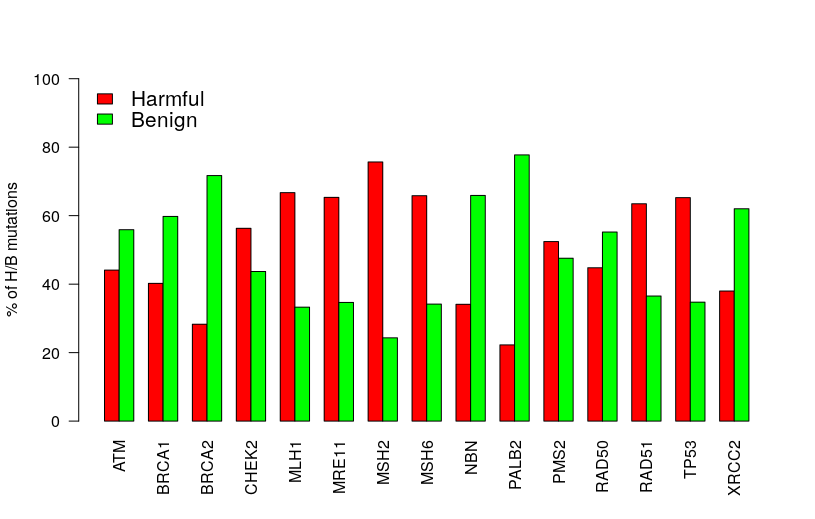
\includegraphics[width=16cm]{img/mutations_per_gene}
\end{center}
\caption{Harmful/benign distribution per gene}
\label{fig:fig-eg}  
\end{figure}

\section{Characteristics and Traits of the Predictions}

Taking into account the predictions of the 11 tested methods, a global score, Harmfulness Index (HI), was calculated. The methods had different prediction traits, depending on their design. The individual contributions of each method can be seen in Figure 3.2. Overall, CADD was the method that predicted more harmfulness, with a value of 71.17\% of the whole dataset. On the other hand, the method that provided the lowest value was MetaSVM, predicting harmfulness for only 28.65\% of all the mutations.

\begin{figure}
\begin{center}
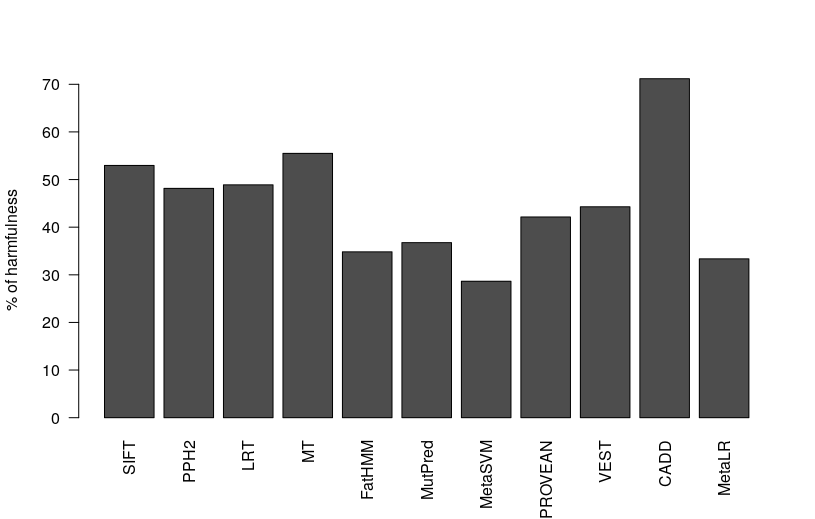
\includegraphics[width=14cm]{img/contribution_per_method}
\end{center}
\caption{Percentage of harmfulness predicted by each method}
\label{fig:fig-eg}  
\end{figure}

The predictions of each method varied greatly for each gene, as seen in Table 3.2. Interestingly, the only method that predicted both extreme overall values for different genes was FatHMM, giving a method score of 0 for PALB2 and of 100 for TP53, followed closely by MetaSVM (0 and 96.23) for the same genes, respectively.

\begin{sidewaystable}
    \centering
    \begin{tabular}
{|r|c|c|c|c|c|c|c|c|c|c|c|c|}\hline\hline
Gene&SIFT&PPH2&LRT&MT2&FatHMM&MutPred&MetaSVM&PROVEAN&VEST&CADD&MetaLR&HI\\\hline
ATM&53.40&39.54&65.91&62.61&12.53&36.25&19.18&37.39&52.67&85.67&19.93&44.10\\
BRCA1&52.82&45.58&14.41&31.94&63.93&19.45&34.45&48.15&25.00&51.42&55.30&40.22\\
BRCA2&48.23&54.35&19.29&21.00&15.28&24.75&13.53&28.64&18.38&52.20&15.50&28.29\\
CHEK2&55.11&50.22&71.75&82.63&26.76&56.51&34.38&49.88&64.66&89.22&38.17&56.30\\
MLH1&56.51&49.11&72.29&84.20&98.08&47.63&52.39&56.37&74.85&82.85&59.60&66.72\\
MRE11&58.67&56.16&82.96&91.48&51.73&59.27&47.80&54.58&68.21&94.13&53.81&65.34\\
MSH2&56.37&55.28&78.67&91.10&99.81&70.54&68.00&61.24&78.02&94.21&79.26&75.68\\
MSH6&56.30&52.49&68.70&86.04&88.88&55.44&54.88&49.96&60.02&87.16&64.30&65.83\\
NBN&53.90&45.31&35.47&46.81&4.09&30.99&16.71&33.35&29.78&61.84&16.82&34.10\\
PALB2&48.03&41.27&18.65&21.60&0.00&9.19&0.00&40.90&21.24&43.98&0.00&22.26\\
PMS2&55.81&50.92&58.28&66.20&26.87&45.13&44.19&53.01&56.26&66.92&53.16&52.43\\
RAD50&53.84&42.25&84.95&91.19&0.60&29.87&1.31&36.93&60.29&90.13&1.33&44.79\\
RAD51&65.72&53.88&93.47&99.30&1.87&71.67&32.35&71.99&86.56&99.52&21.80&63.47\\
TP53&52.81&53.32&44.52&65.43&100.00&54.80&96.23&40.96&44.14&68.56&97.04&65.26\\
XRCC2&51.09&43.07&55.43&64.66&2.06&38.45&7.85&36.23&42.90&69.78&6.23&37.98\\\hline\hline
    \end{tabular}
    \caption{Average harmfulness scores per method for each gene}
\end{sidewaystable}

The methods were classified into three groups to explore the different traits of their design principles and their contribution to the overall consistency of the predictions. Similar trends were observed in the three groups, showing a clear positive correlation between the predicted HI and the Grantham distances corresponding to the amino acid substitutions. The correlation patterns can be seen in Figure 3.3.

\begin{figure}
\begin{center}
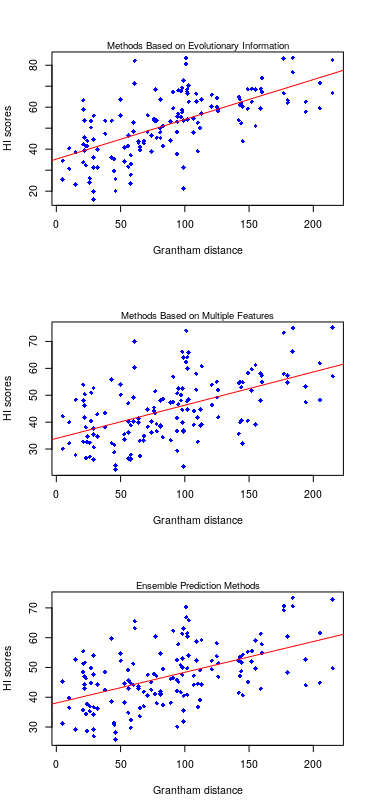
\includegraphics[width=10cm]{img/scatter_plots}
\end{center}
\caption{HI scores and Grantham  distances for each group of methods}
\label{fig:fig-eg}  
\end{figure}

\subsection{Methods Based on Evolutionary Information}

The first group was composed of the methods that are strongly based on evolutionary information of the sequences to predict their deleteriousness: SIFT, LRT and PROVEAN. The first group was composed of the methods that are strongly based on evolutionary information of the sequences to predict their deleteriousness: SIFT, LRT and PROVEAN. These methods tended to show a slightly more strong correlation between HI and Grantham distances, and provided higher HI values. The top 5 HI scores all correspond to a Tryptophan replacement, and are all above 80. The bottom scores involve different types of replacements, all of them having Grantham distances below 100. The predictions provided by SIFT showed the highest values of harmfulness in the group with an overall score of 52.96, followed closely by LRT and PROVEAN.

These methods emphasize evolutionary data to predict the harmfulness of the variants. Based on the slightly higher proportion of harmfulness predicted by the methods, a possible explanation would be that incorporating other types of information such as genome annotations, GC content and methylation levels (used by other methods) could reduce sensitivity for the current dataset.

\subsection{Methods Based on Multiple Features}

The second group was composed of methods that are based on a combination of all sort of features and techniques to predict the deleteriousness of variants: PolyPhen-2 (PPH2), MutationTaster (MT2), FatHMM, MutPred and VEST. The results also show a clear correlation between the HI predictions and the Grantham distances, although with overall lower harmfulness values compared to the previous group, and more similar to the global trend. The top HI values also correspond with Tryptophan replacements, as in the case of methods based on evolutionary information, but with scores roughly 10 points lower than in that group, between 70 and 76.

Several features are incorporated in these methods to enrich or adjust their predictions. Their results suggest a less sensitive overall trend in their predictions, and also more in line with the general results of the third group and the global trend. The highest HI was given by MT2, which had an overall HI score of 55.50, and the lowest one was provided by FatHMM (34.83).

\subsection{Ensemble Prediction Methods}

The third group included the ensemble prediction methods, which were suitable to be examined separately due to the fact that they incorporate several of the already mentioned scores in their predictions, along with many other biological features from several data sources. There are three methods in this group: CADD, MetaSVM and MetaLR, the last two being the machine learning-based ensemble predictions provided by the dbNSFP. This was by far the most diverse group, having provided both the lowest and the highest overall HI scores in the whole group. One extreme was represented by CADD, that had an HI value of 71.17, and the other by the two dbNSFP methods, which had the two lowest values globally, 28.65 for MetaSVM and 33.35 for MetaLR. One important aspect of CADD is that it doesn't provide a categorical classification as most of the other methods. Instead, several different scores are provided to suit different needs. The main `raw' score is the immediate output of the model, but it does not hold an absolute meaning and it is not comparable with other scores. In the context of this study, the `phred-like' score provided is used. The authors' recommendation is to use this score for purposes of comparison and when a cut-off value has to be put in place. Even for such cases, it is stated that the ideal value varies depending on the context (Rentzsch et al., 2019). A value of 20 was used, taking into consideration the range of 10-20 recommended by the authors and using the least restrictive value (mutations with a score higher than 20 were considered harmful). Even with this configuration, the CADD method labelled more variants as deleterious than any other method.

The other two methods deploy similar approaches, using the same dataset (dbNSFP) as a source for training their machine learning models, and differing only in the particular type of algorithm used. These methods also incorporated several of the other assessed methods, but different from CADD, they provide precalculated categorical values for tolerance/deleteriousness.

The considerable difference between these two different ensemble-like approaches could be explained in terms of the set of biological features incorporated in each one (only a subset of them is common to both) and the training datasets of their respective algorithms. The observed different behaviour of the CADD method suggests a consistency with previous benchmarking efforts, in which some methods with much fewer components scores performed better in making predictions for the chosen dataset (Dong et al., 2015). This highlights some of the challenges regarding the building of diverse large high-quality datasets in machine learning approaches. Having both extremes within the same class, however, kept the group overall scores from deviating too much from the global prediction tendency.

\section{Global Consistency and Prediction Trends}

To assess the general consistency of the prediction values of all the assessed methods, HI values were computed for each generated variant and summarised following different criteria to identify patterns of consistency and disagreement among all the tools.

\subsection{Mutation Frequencies and Grantham Scores}

Of the total possible Grantham distance scores estimated for the different types of potential amino acid substitutions, which range from 5 to 215, 150 were assigned to at least one variant for the generated dataset. It should be pointed out that some Grantham distance values are shared among different types of amino acid substitutions. Also, in the context of the current work, interchanges between a pair of amino acids and their opposite direction counterparts were treated separately. After the variants curation, a summary of HI scores for the 150 different types of mutations observed in the dataset was constructed.

The most and least observed mutation types are depicted in Table 3.3. By far, the most observed type was a substitution of a Glutamic acid for an Aspartic acid, which was observed 2763 times and has a Grantham score of 45 (located in the lowest quartile of the possible range), and its counterpart was observed 1648 times, almost only half of that value. Both Glutamic acid and Aspartic acid have two codons that code for the amino acid, so this is probably related to their higher frequency in the protein. Despite the difference in number, the predicted HI values were very similar, with 31.15 in the first case and 33.62 in the second one. The other most commonly observed mutation types, Lysine/Asparagine, Phenylalanine/Leucine and its counterpart, and Serine/Arginine, all had HI values below 50 (probably benign). On the opposite extreme, substitutions of a Serine for a Tryptophan, with a Grantham score of 177 (upper third quartile of the range), were observed only 25 times in the whole dataset. This is likely a reflection of the fact that, despite Serine has six different corresponding codons, a transition to a Tryptophan with a single nucleotide change is only possible in one case. Its counterpart substitution was also rarely observed, 119 times in total. The predicted HI was high in the former case and very high (within the top 5 HI values) in the latter. Other very rarely observed mutation types were Threonine/Methionine and the replacement of an Arginine for a Histidine, Cysteine or Glutamine, all with HI values above 50 (probably harmful), except the first one.

\begin{table}
\begin{center}
\begin{tabular}{|c|c|c|c|}\hline\hline
Mutation&Count&Grantham distance&HI\\\hline
Glu to Asp&2763&45&31.15\\
Lys to Asn&2506&94&42.75\\
Phe to Leu&1835&22&49.47\\
Leu to Phe&1704&22&49.97\\
Ser to Arg&1663&110&36.55\\\hline\hline
\end{tabular}
\begin{tabular}{|c|c|c|c|}\hline\hline
Mutation&Count&Grantham distance&HI\\\hline
Ser to Trp&25&177&63.27\\
Thr to Met&25&81&41.45\\
Arg to His&74&29&55.04\\
Arg to Cys&80&180&60.80\\
Arg to Gln&96&43&57.39\\\hline\hline
\end{tabular}
\end{center}
\caption{Most and least observed mutations}\label{wombat}
\end{table}

The highest and lowest predicted HI scores can be observed in Table 3.4. The lowest global score was predicted for a substitution of a Serine for an Asparagine, which has a Grantham score of 46 (first quartile of the range). The other mutation types with very low scores, Asparagine/Serine, Valine/Isoleucine and its counterpart, and, Serine/Alanine all had Grantham scores within the first quartile, except the last one. Globally, the predicted most harmful substitution (HI 77.85) corresponded to a replacement of a Tryptophan for a Cysteine, which, as expected, has the highest Grantham score possible (215), and was observed 236 times in the dataset. All the mutation types within the top 5 of HI scores involve a replacement of a Tryptophan (for a Glycine, Arginine, Serine and Leucine, respectively), and have HI scores above 70.

\begin{table}
\begin{center}
\begin{tabular}{|c|c|c|c|}\hline\hline
Mutation&HI&Grantham distance&Count\\\hline
Trp to Cys&77.85&215&236\\
Trp to Gly&77.58&184&120\\
Trp to Arg&76.89&101&238\\
Trp to Ser&76.39&177&119\\
Trp to Leu&73.80&61&119\\\hline\hline
\end{tabular}
\begin{tabular}{|c|c|c|c|}\hline\hline
Mutation&HI&Grantham distance&Count\\\hline
Ser to Asn&24.57&46&538\\
Asn to Ser&24.82&46&756\\
Val to Ile&25.23&29&600\\
Ser to Ala&25.93&99&909\\
Ile to Val&26.04&29&802\\\hline\hline
\end{tabular}
\end{center}
\caption{Most and least harmful mutations}\label{wombat}
\end{table}

The opposite extremes of the HI range indicate agreement; very high values indicate consistency among the methods in predicting harmfulness, while very low scores indicate agreement towards predicting benignness. Values near the middle of the range indicate the worst consistency, meaning ambiguity in the predictions. Types of mutation with very low level of consistency are Glutamine/Proline, Leucine/Phenylalanine, Isoleucine/Threonine, Isoleucine/Arginine and Methionine/Lysine, all of them with HI values slightly below or above 50. Their frequency in the dataset varies a lot, and their Grantham scores are distributed throughout the first and second quartiles of the range and, but without being too low.

\subsection{HI and Consistency Distribution}

The results produced by all the evaluated methods indicate, in all cases, a clear positive correlation between the predicted HI score and the Grantham distances. In addition to this, it was desirable to establish if a pattern existed within the levels of consistency achieved by the methods throughout the range of Grantham score values. A working hypothesis was that the level of consistency would be higher for more extreme prediction values.

To evaluate this, the range of possible Grantham scores was divided into three equal-sized tiers (lower/mid/upper), grouping the HI levels in each tier. The level of consistency are represented in Figure 3.4.

\begin{figure}
\begin{center}
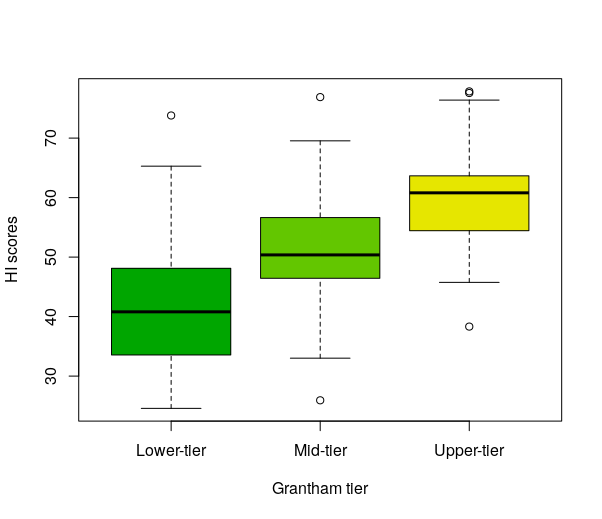
\includegraphics[width=11cm]{img/boxplot}
\end{center}
\caption{Consistency levels per Grantham tier}
\label{fig:fig-eg}  
\end{figure}

For the lower Grantham tier, the minimum and maximum values were 24.57 and 73.80, respectively. The values for the first and third quartiles were 33.59 and 48.08, with an interquartile range (IQR) of 14.49, the highest among the three tiers. The IQR in this context indicates how broad is the spectrum of agreement between the different methods within that tier. The median value was 40.80, appearing at only 0.45 points from the average value for the tier, indicating consistency in favour of a benignnes prediction.

The second Grantham tier had min/max values of 25.93/75.89, and an IQR of 10.13 between first and third quartiles (46.45 and 56.58, respectively), a lower value than in the lower Grantham tier. The median value was further away from the tier's mean, at a lower value of 50.37, but very close to the global value of complete disagreement in HI prediction.

Lastly, the upper Grantham tier had an IQR value of 7.84, having the values of 55.63 and 63.47 as first and third quartiles and 77.85 (the highest HI value) and 38.32 as maximum and minimum values, respectively. The median value is above the average value for the tier (60.80). The IQR of the tier was the smallest among the three tiers, indicating a higher degree of consistency among the predictions of different methods.

From the values obtained for each tier, it can be established that a higher benignness value does not involve a greater consistency among the predictions, despite there is a clear tendency to label the mutations as benign. On the other had, a much greater consistency among the tools was observed with higher harmfulness values, with the IQR value of the upper-tier being reduced more than half of the value for the lower one.

\subsection{HI and Location of the Missense Mutations}

Having calculated the harmfulness values for each type of mutation and per gene, another possible differentiating factor explored was the location of the particular location of the missense mutation in relation to the protein’s coding sequence.
As with the Grantham values, the variants were grouped into different equal-sized tiers, representing the different regions of their coding sequence in respect to the N-terminus of the protein (start/lower mid/upper mid/end), and the HI values for each group were calculated. The distribution can be seen in 3.5.

\begin{figure}
\begin{center}
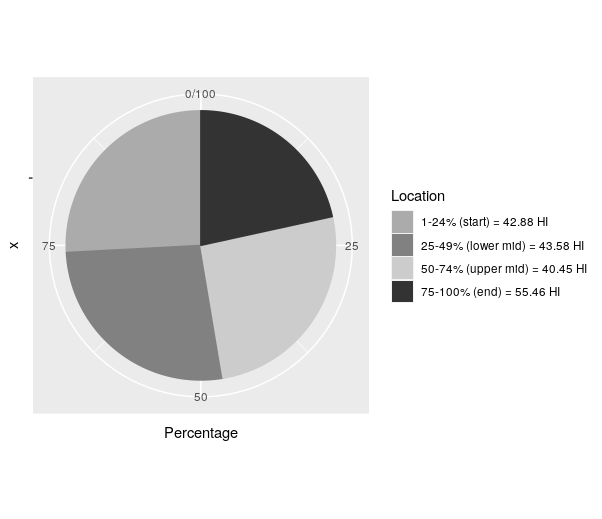
\includegraphics[width=14cm]{img/pie}
\end{center}
\caption{HI scores per location in coding sequence}
\label{fig:fig-eg}  
\end{figure}

The lengths of the coding sequences are within a range of 843 nucleotides for XRCC2 to 10257 for BRCA2. As shown in the chart, the amount of generated mutations had a very balanced distribution, with values of 25.84\%, 26.80\%, 25.79\% and 21.57\% for the start, lower mid, upper mid and end location tiers, respectively. The distribution of HI values among each tier was slightly more varied. The highest predicted HI values were found in the end tier with an HI value of 55.46, followed by the lower mid tier, that had a value of 43.58. The start and upper mid tiers had the lowest values, 42.88 and 40.45, respectively.

Despite the modest variation of HI values among the different location tiers, the difference could be explained by mere chance.

\subsection{HI and Gene Missense Change Tolerance Values}

The Z-scores corresponding the chosen set of genes were obtained from the gnomAD database and incorporated to the analysis. The values are within a range of -2.78 to 2.62. The results comparison between global HI scores with Z-scores can be seen in Table 3.5.

\begin{table}
\begin{center}
\begin{tabular}{|r|c|c|}\hline\hline
Gene&HI&Z-score\\\hline
ATM&44.10&1.105\\
BRCA1&40.22&0.582\\
BRCA2&28.29&-1.289\\
CHEK2&56.30&-0.450\\
MLH1&66.72&-0.304\\
MRE11&65.34&0.130\\
MSH2&75.68&-2.449\\
MSH6&65.83&-2.780\\
NBN&34.10&0.609\\
PALB2&22.26&0.276\\
PMS2&52.43&-0.557\\
RAD50&44.79&1.250\\
RAD51&63.47&2.622\\
TP53&65.26&0.983\\
XRCC2&37.98&-0.127\\\hline\hline
\end{tabular}
\end{center}
\caption{HI values and Z-scores per gene}\label{wombat}
\end{table}

The values do not seem to be correlated, apart from the noticeable case of the MSH2 gene, that having the highest overall HI score among all the genes also has the second-lowest Z-score, meaning the number of different missense variants observed in the transcript where much more than expected. But it is likely that a larger set of genes an a more detailed comparison would be needed to obtain conclusive results.

One thing to notice is that, for this comparison, it was not possible to obtain the Z-scores of the particular MANE transcripts selected for this study, and values corresponding to other reference transcripts of the same genes in the database had to be used. That could also have an influence on the observed results.

\section{Discussion}

Motivated by some concerns and limitations in the way the characteristics of different pathogenicity prediction methods are usually compared and explored, this project followed a more theoretical approach and worked with the complete dataset of possible mutations for 15 sample genes. This allowed to construct a bigger and more diverse dataset, and allowed a better separation between the examined data and the individual traits and characteristics of the different predicting tools with a range of different types of mutations.

Different pathogenicity prediction approaches were selected and evaluated, based on their popularity, free access, and availability as web-based services that could be integrated into an automated pipeline, to achieve a better reproducibility of the dataset. The 11 selected prediction methods provided a wide sample of different computational approaches in pathogenicity prediction.

Of an original raw dataset of 117840, it was possible to keep 104267 variants with predictions from every assessed method, which was still a large dataset for the scope of the study. A general prediction was then calculated and summarised in different ways to explore the patterns of consistency among approaches that occasionally differed a lot in their design principles.

Different harmfulness prediction principles were assessed and compared to explore the patterns of their results. Two patterns were identified: Firstly, methods that emphasised the use of evolutionary data in their pathogenicity predictions tended to produce higher estimates of deleteriousness than those incorporating other diverse biological factors, annotations from several sources and more complex algorithmic approaches. Secondly, ensemble methods taken individually showed both extremes in their harmfulness prediction, with the dbNSFP machine learning-based methods producing the lowest HI scores and the CADD ensemble method producing the highest. Taken as a group, the methods produced results very similar to the general trend. The top and bottom global HI scores corresponded to CADD and MetaSVM, respectively. It was observed that when the methods incorporated a very high number of biological factors into their design, the predictions tended to be more extreme, and additional decisions have to be made to determine the correct parameters and cut-off values for each particular research context.
The levels of agreement among tools were examined with respect to the Grantham distance values assigned to each type of mutation. This allowed to the identification of, first, a clear positive correlation between the predicted harmfulness values assigned to the mutations and a greater Grantham distance, and second, a very noticeable trend in the consistency of the results, namely, a progressive increment in consistency among the tools for higher Grantham distances. This result could potentially have an impact on the way pathogenicity tests are currently performed.

The exploration of possible patterns of traits in respect to the harmfulness of mutations occurring in particular regions of the protein's coding sequence did not show particular trends to examine further, due to the fact that the differences between the number of mutations occurring in each differentiated region are very similar. An alternative might have been to look at predictions occurring within protein domains.

Similarly, no apparent relation was found while contrasting the global predicted harmfulness scores with the levels of mutation tolerance assigned to the respective proteins in the gnomAD's project database. It is possible that some other prediction methods (or some of the evaluated ones but working with specific datasets) that were built prioritising the same biological features to those used by the gnomAD database could produce results in correlation to gnomAD's Z-scores, but to establish this it would be more appropriate to extend the set of genes as much as possible to allow for conclusive results.

It must be acknowledged that, as it is common in projects of similar nature, the results and conclusions presented rely unavoidably on a series of assumptions and simplified models of complex biological processes. This was particularly true of the approach taken in this work, given that it was based on a computationally generated dataset and depended greatly on possibly arbitrary decisions in regards to cut-off scores and other criteria used to differentiate benign and harmful mutations. At the same time, despite the fact that the selected tools had dissimilar design principles and techniques, their results cannot be treated as completely independent from each other, due to frequent overlap among them, which is particularly true of the ensemble scoring methods.

Limitations of the project included both computational and biological aspects. In contrast with the scarce availability of real high-quality datasets that could be used as reference and training for new algorithmic approaches, there is a huge number of available prediction tools for pathogenicity. Some are more specialised in particular biological contexts and others incorporate broader prediction aspects. The first challenge for work of this nature is the gathering of the greatest amount of prediction inputs as possible. This can sometimes be difficult due to the wide range of platforms and formats used for the deployment of the tools. The dbNSFP database and the Ensembl Variant Effect Predictor provided a highly flexible gateway to access the predictions of most of the main tools, which was taken advantage of within the context of this work. However, many state-of-the-art tools do not provide a simple way to perform high volume predictions, such as the ones necessary for this project. Moreover, in some cases, new prediction values corresponding to improved versions of the methods or trained with newer datasets were available in the particular platforms of each tool but not immediately updated in the dbNSFP due to their incomplete nature. The selected tools included most of the most commonly used methods and gave a diverse sample of prediction approaches, but this selection was of course incomplete. At the same time, the need to retrieve all the prediction information for each of the generated variants involved several hours of running time for the designed software, which limited the gene sample to the 15 chosen genes for the current project.  The work was also understandably limited by biological factors, given that an empirical validation of such large scale would not be feasible, which is a recurrent constraint in the development and assessment of many implementations of computational biology projects. However, the observed results can provide a good complement for more empirical research programmes.

\section{Evaluation}

The assessment of the results obtained from the described analyses differed from the usual evaluation methodologies implemented in the related literature in two ways. First, a common approach used for the assessment of the results in similar studies is to find curated datasets of known pathogenicity that are considered independent from the ones used for the training or development of the new methods, and subsequently compare the generated predictions with those of the chosen dataset. Thus, a statistical comparison can be performed using the predicted and the ground truth values to get a similarity score. But this kind of evaluation is not feasible in the context of this work due to the lack of ground truth values for the vast majority of the generated dataset, with the possible exception of particularly well-studied genes like BRCA1 and BRCA2. If a restrictive methodology had been applied and the dataset had been reduced to only include predictions for which ground truth values are known, its size would have been reduced considerably and the mentioned issues of circularity between training and testing datasets would have reappeared. Second, as the HI scores calculated in this work are not used to test a new prediction strategy but to measure the consistency between existing methods, its values were not independent of each of the selected method's values, and consequently were not comparable for benchmarking purposes.

As an exploratory work that was focused on identifying possible correlations or traits among the different prediction methods, the criteria to critically assess the quality and relevance of its observations leaned towards generating enough data that could provide a strong basis to the observed patterns, establishing parameters for the reduction of ambiguity or incompleteness of this data, and the use of the Grantham scores as an external independent estimator of the variants' harmfulness. A size of 100000 different variants after data curation was established as a desirable minimum, and variants with null or ambiguous values for at least one of the prediction methods were excluded.
Working with a computationally generated dataset had several advantages. First, it provided an equally levelled ground for all the methods, which eliminates the problem of correctly selecting the datasets that could show the real overall trends of each one. And second, it is not limited by the range of empirically observed variants or distorted by over-representation of certain genes above others. However, these aspects also constitute its disadvantages, particularly in terms of empirical validation.

In regards to the software developed in support of the research, it can be critically evaluated considering many different aspects. If compared with similar applications provided to integrate several pathogenicity prediction methods, two main aspects stand out. The first one is that the dynamic generation of the dataset to be evaluated. Due to their different aims, it is usual with most tools that the variant dataset has to be provided by the user following a particular format, or in a few cases, chosen from very limited subsets of variants from curated datasets. In this case, only a set of gene symbols has to be specified, and the coding sequence retrieval, variants generation and prediction retrieval are performed automatically. This means that if the project were to be expanded with more genes, the additional variant data could be easily generated. The second one is the capacity to handle high volumes of data. Due to the asynchronous implementation of the two main parts (generation and prediction retrieval) and the  possibility of separating genes in different batches, it is fairly simple to generate and handle the complete list of mutations for a set of genes. Another design advantage of the tool is its accessibility. It has a fairly simple user interface, and as it is completely web-based, it can be accessed from any pc with an internet connection. Lastly, it was developed with extensibility in mind, up to date technologies and with an open-source license.

One disadvantage of the tool is that, as it uses internet-based resources like the Ensembl Variant Effect Predictor, its performance is limited by the usual constraints of web tools when handling data. A different approach that would considerably improve the tool's performance would be to implement all the prediction tools in a dedicated server, which would eliminate the necessity of using external tools. However, apart from the increased complexity that such implementation would have, it would also mean that the predictions would have to be performed each time new versions are launched or new genes and features are added, as opposed to the updated precomputed values that the VEP provides.

\chapter{Conclusion}
\label{cha:conclusion}

An important task for current bioinformatics is to provide computational models and tools to take advantage of the increasing amount of information provided by the continuous sequencing and annotation of genomes in all forms and contexts. These tools are particularly useful in emerging areas as biomedical engineering, diagnostic testing and personalised medicine, which rely heavily on genomics to predict and treat diseases. The prediction of levels of pathogenicity of single nucleotide polymorphisms on protein function plays an important role in this context, and several tools and methods are available for the task, tested and trained with different datasets and emphasising different aspects in their predictions. While several previous efforts have made surveys of these methods, summarised their features and compared their performance using particular datasets, a frequent challenge faced by them is to find datasets with non-overlapping data to establish the quality of the results. This study used a different approach, using a computationally generated dataset of all the possible SNP variants for a set of genes and examining the patterns of prediction of several tools.
Several aspects were explored, including prediction traits produced by particular approaches, global predicting values, the relationship of the predicted pathogenicity with the Grantham distance scores of the mutations involved, predicting traits according to the location within the coding sequence and the relationship of the results with global tolerance levels for missense mutations of the proteins, provided by external databases.

The exploratory approach and the supporting tools adopted for the project have proven fruitful and have helped to meet the project aims thoroughly. The size of the generated dataset facilitated the examination of individual and global patterns in the results of the different methods. In addition to the observation that the predicted levels of pathogenicity of the variants correlate positively with the Grantham distances corresponding to their amino acid replacements, it was determined that the levels of consistency of the predictions between different tools increased with higher values of harmfulness, which was not observed in the opposite case (higher benignness values).
At the same time, an effective support tool was created to serve as a platform to extend the study to consider more genes and prediction methods and to provide an easy and automated way of replicating the dataset for future projects.

In the light of previous studies and the general context of the research on the clinical significance of SNVs and the possibilities of in silico predictions as the first step towards promising areas such as personalised medicine, the present work provides very interesting insights about the traits of deleteriousness prediction methods and shows that a purely theoretical/computational approach can provide useful complementary information in empirical research projects. Moreover, the Harmfulness Index values calculated for the generated variants can be used as reference values to benchmark new methods and tools.

The obtained data and outcomes from this work throw light on several new possible lines of further research and extensions to the project's scope, both in terms of biological features and additional computational support. In addition to the already investigated biological aspects, a very interesting addition would be the incorporation of data from protein family databases such as Pfam or PROSITE to explore possible patterns of pathogenicity prediction within particular protein domains. Another important addition would be the inclusion of as many genes as possible in the dataset to allow for a full comparison with the set of missense mutation tolerance values from the gnomAD database. This would allow for a more thorough investigation of possible existing correlations among the predicted pathogenicity values for the genes and the empirically observed tolerance values. Additionally, different amino acid replacement scoring methods could be considered in comparison with the Grantham score, such as Sneath's index (Sneath, 1966) or Miyata's distance (Miyata et al., 1979). 

From a computational point of view, several improvements and optimisations could be added to the developed support tool. A highly useful feature would be the possibility to export the final dataset in several different formats and levels of detail. Due to the relatively high execution time necessary, this could be implemented as an asynchronous process that submits the data to a specified email. Another interesting addition would be to provide the graphs, tables and charts generated for the current work automatically in an overview page, accessible once the processing is finished. Furthermore, and based on the extensive research and use of the Ensemble REST API to access resources like the dbNSFP database in an effective way in the context of this work, it would be very desirable to implement a set of similar features like a REST-based interface for integration with other services and tools and the provision of precomputed values that facilitate access for data-intensive tests and applications.

In summary, this project has proven to be a fruitful opportunity to develop and apply computational tools to compare, integrate and explore both well-known and cutting edge methods for SNV pathogenicity prediction, and provided both a rich computationally generated dataset and an easy to use open-source application to help to replicate the described results and also serve as a support tool for similar projects in the future.

\section{Conflict of Interest}
The author declares that he has no conflicts of interest.

\bibliographystyle{apalike}
\nocite{*}
\bibliography{refs}

\end{flushleft}
\end{document}
